\documentclass[border=2pt]{standalone}
\usepackage{tikz}
\begin{document}
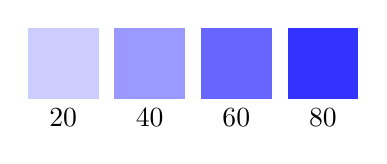
\begin{tikzpicture}
  \foreach \x in {1,3,5,7} {
    \fill[blue!\the\numexpr\x/2*20\relax] (\x*0.55,0) rectangle ++(0.9,0.9);
    \node[below] at (\x*0.55+0.45,0) {\the\numexpr\x/2*20\relax};
  }
\end{tikzpicture}
\end{document}
